\chapter{Modellierung}
\label{sec:modellierung}
Basierend auf dem Trainingsziel werden die Zyklen mit spezifischer Gewichtung gestaltet. Dabei sind Belastungs und Regenerationsphasen einzuplanen. Danach fließt in der Phase der konkreten Trainingsplanung die Anforderung und das individuelle Belastungsprofil des Sportlers ein. Regenerationsphasen müssen berücksichtigt werden. 
In der letzten Phase werden die konkreten Trainingseinheiten festgelegt. Diese beinhalten sowohl Trainingsmethoden, als auch Intensität und Dauer der Belastungen. 
Diese Arbeit behandelt ausschließlich die initiale Erstellung eines Trainingsplans. Es erfolgt keine Trainingssteuerung durch Dokumentation oder Kontrolle.

Die Anforderungen aus der Trainingswissenschaft bilden als mathematisches Modell die Grundlage für den Algorithmus. 

\section{Übersicht}
\label{sec:modellierung:uebersicht}
    \begin{figure}[tbh]
    	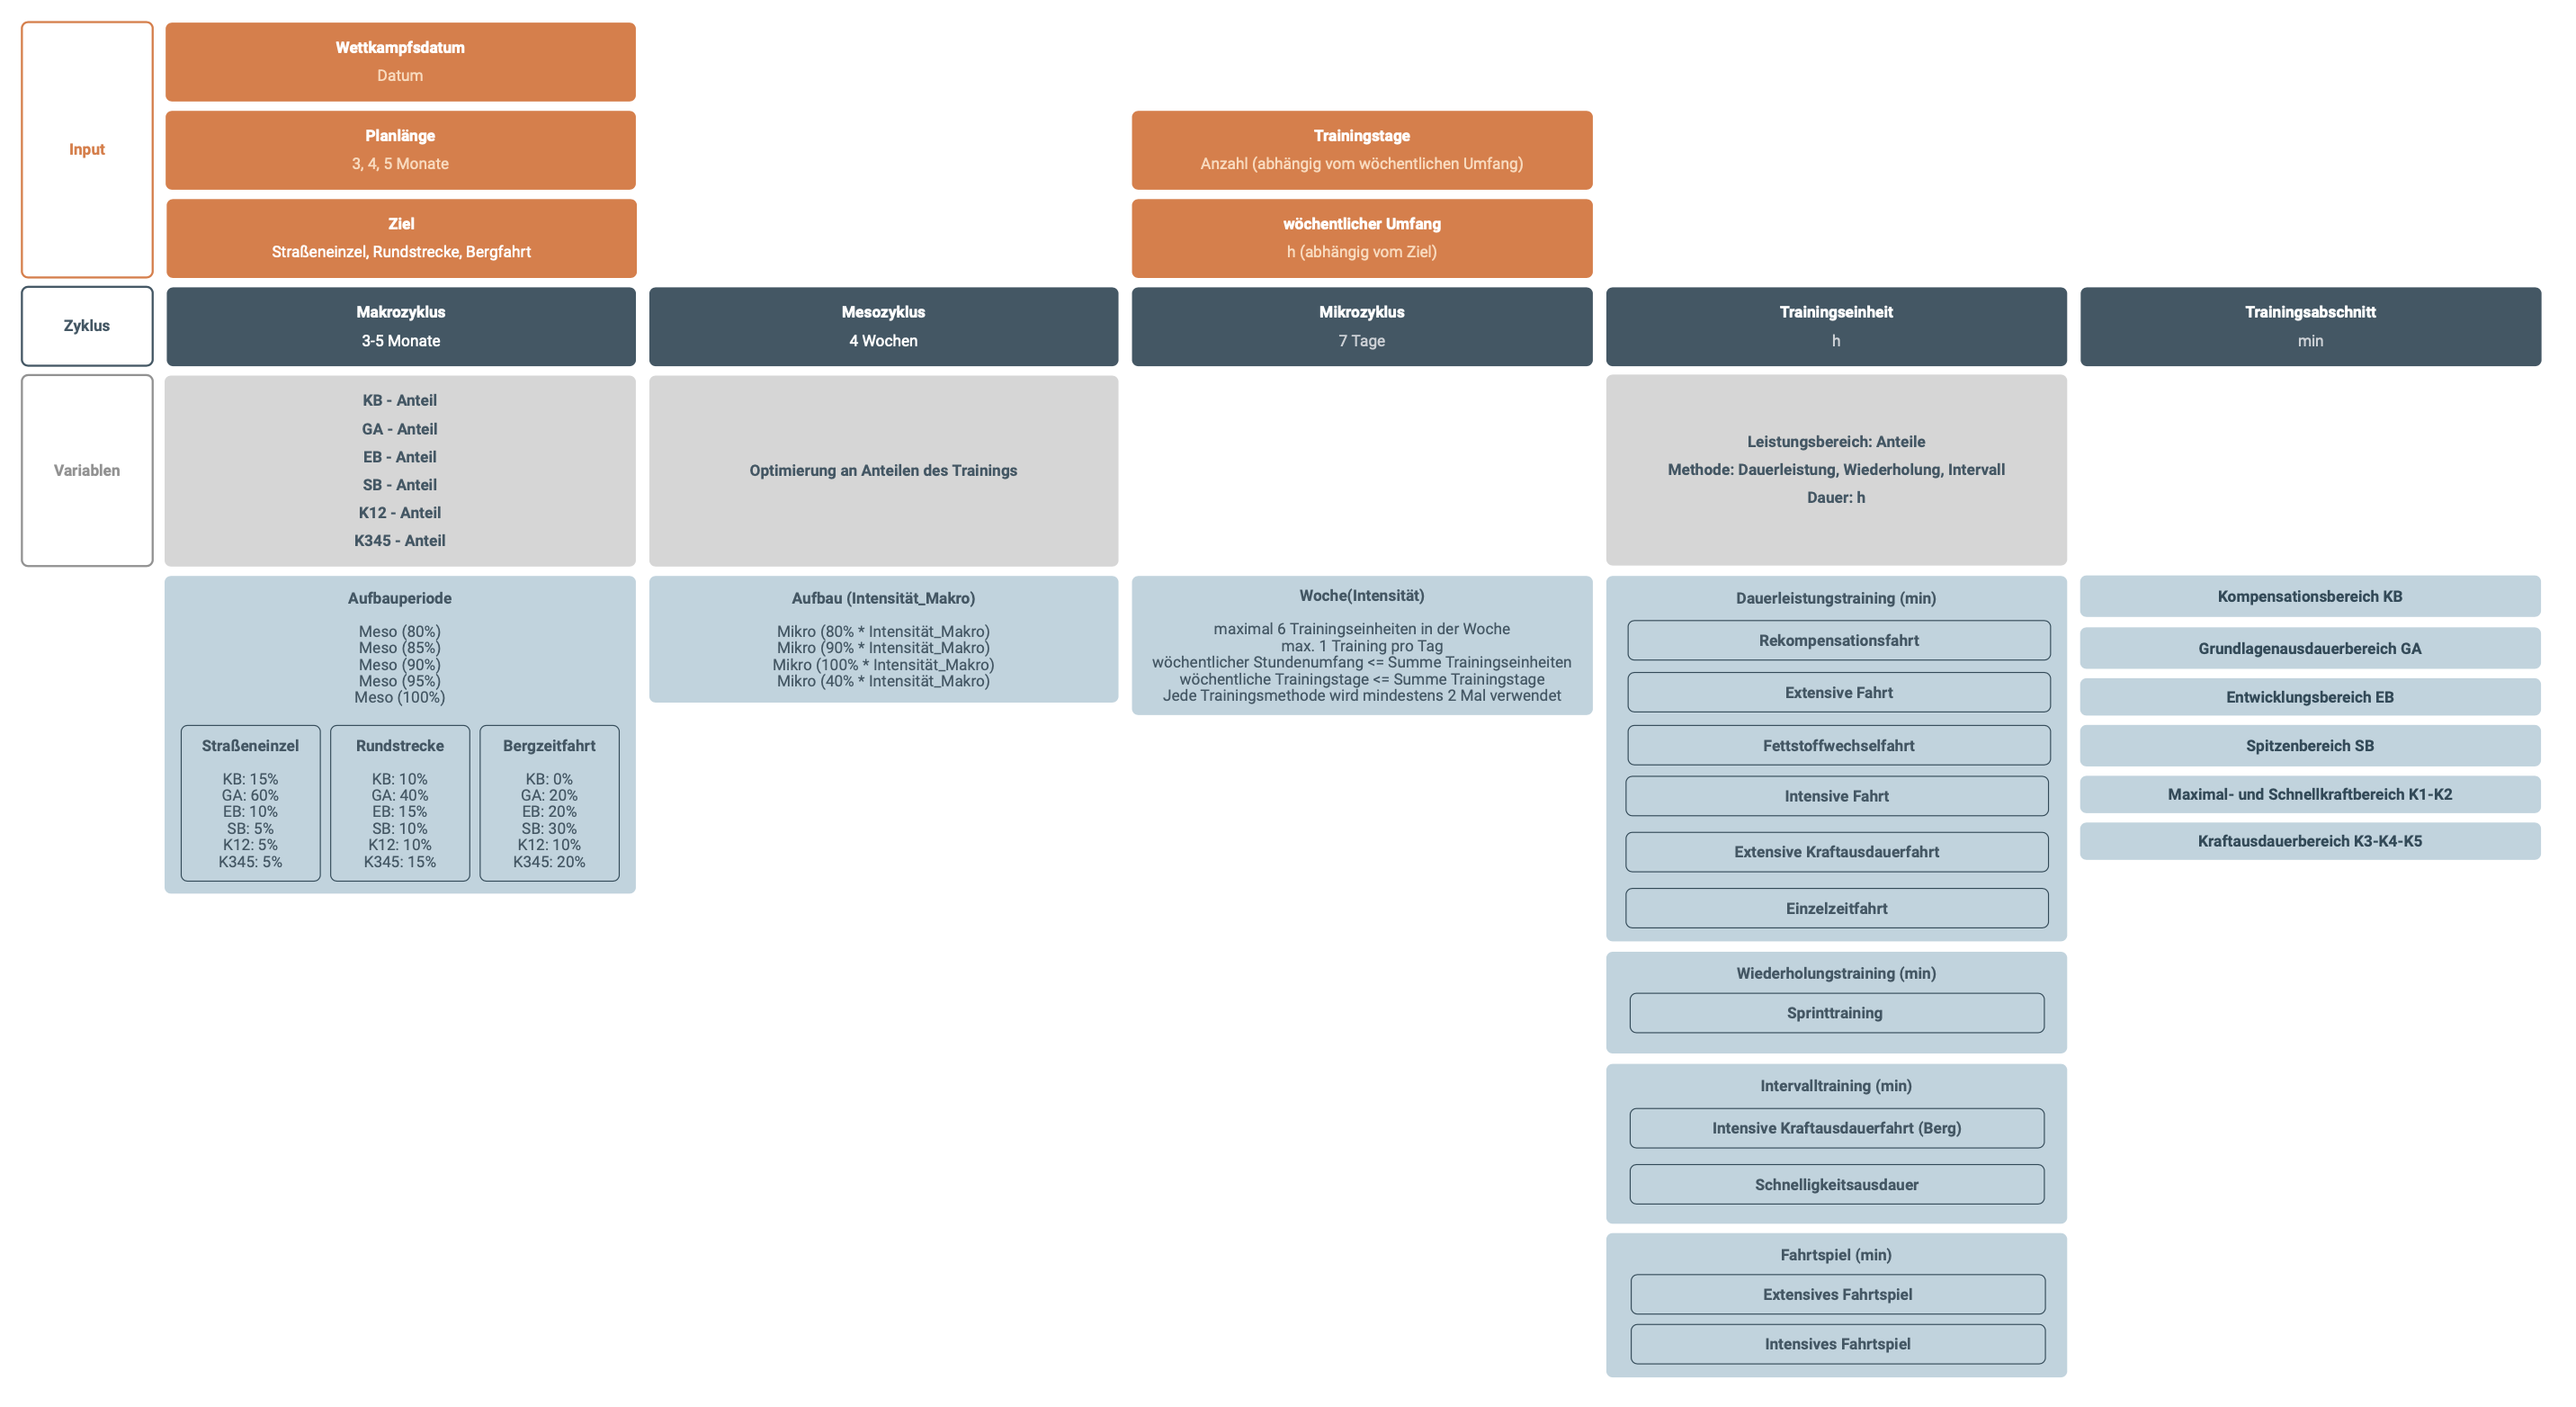
\includegraphics[width=\textwidth]{gfx/modellierung.png}
    	\caption{Schema aus Makro-, Meso- und Mikrozyklen}
    	\label{fig:modellierung:schema}
    \end{figure}
    
Bei der Erstellung eines Trainingsplans wird auf die Constraint Programmierung zurückgegriffen. Dennoch ist der Solver in ein Programm eingebettet, dass bereits die Eingabe und Ausgabe des Benutzers handhabt. Die Validierung von Eingabe und Ausgabe ist so unabhängig von der Modellierung mit Constraint Programmierung. Die Optimierung ist auf Ebene der Mesozyklen implementiert. So wird jeder Monat unabhängig der anderen modelliert. Gesteuert wird die Gewichtung der Leistungsbereiche in den einzelnen Monaten durch zwei Faktoren. Die Länge des Plans (3, 4 oder 5 Monate) bestimmt die Anzahl der Mesozyklen. Desweiteren steigt bei Mesozyklen die Gewichtung der wettkampfsspezifische Ausdauer proportional \TODO{Ist das so?} zur Nähe am Wettkampfstermin.
    \begin{enumerate}
        \item Trainingsziel bestimmen
        \item Einfach-Periodisierung des Trainingplans zum Wettkampfstermin
        \item Vierfach-Periodisierung der Aufbauphase aus Vorbereitungsperioden
        \item Constraints auf Ebene der Hierarchie definieren 
        \item Solver erstellt Trainingseinheiten
    \end{enumerate}
    \subsection{hierarchische Zyklisierung}

\section{Designentscheidungen}
\subsection{Kraftbereiche vs. Trainingsmethoden mit Belastungsstufen einer Einheit}
\subsection{Optimierung auf Ebene der Mesozyklen}
    
\section{Model}
\subsection{Konstanten}
In der Modellierung betrachten wir Konstanten gesondert. Diese Größen sind in jeder Lösungsinstanz relevant aber vor der Modellierung festbestimmt. Weitestgehend entsprechen sie den Eingaben des Benutzers.
Input wöchentlicher Trainingsumfang (Stunden)
$max_{hours} \in [0, 40]$

Input Anzahl wöchentlicher Trainingstage
$max_{days} \in [1, 7]$

Input Trainingsziel
$kb \in [0, 100]$
$ga \in [0, 100]$        
$eb\in [0, 100]$
$sb\in [0, 100]$
$k123\in [0, 100]$
$k45\in [0, 100]$
        
Input Wettkampfstag -> Trainingslänge = Anzahl der Tage
$length \in \{ 84, 112, 140\} $ 
        
\subsection{Variablen}
Unter den Variablen der Modellierung versteht man die veränderlichen Größen.

        
        Variable um den Tag der Trainingseinheit $i$ zu identifizieren
        \begin{equation}
            \forall i \in [1, \text{length}], \text{day}_i = [\![1, \text{length}]\!]
        \end{equation}
    
        Variable um Leistungsbereich der Trainingseinheit $i$ zu identifizieren
        \begin{equation}
            \forall i \in [1, \text{length}], \text{range}_i = [\![0, 6]\!] \text{oder} \{\text{KB, GA, EB, SB, K12, K345}\}
        \end{equation}
        
        Variable um Dauer der Trainingseinheit $i$ zu identifizieren
        \begin{equation}
            \forall i \in [1, \text{length}], \text{duration}_i = [\![0, 10]\!]
        \end{equation}
        
        Variable um Trainingsmethode der Trainingseinheit i zu identifizieren
        \begin{equation}
            \forall i \in [1, \text{length}], \text{method}_i = \{\text{DL, IV, WH}\}
        \end{equation}

    \subsection{Constraints}
    \subsubsection{Allgemein}
    Nur ein Training pro Tag
        \begin{equation}
            \forall i, j \in [1, 150]^2, i\neq j \Rightarrow day_i \neq day_j
        \end{equation}
    Summe der Trainingsstunden unter wöchentlichem Umfang
    \TODO{Definition einer einzelnen Woche}
        \begin{equation}
            \forall i = k * 7 + 1, k \in \math{Z}, \sum_{i}^{i+6} \text{duration}_i \leq max_{hours}
        \end{equation}
        \begin{equation}
            \forall i \in \{ i = k * 7 + 1, k \in \math{Z} \}, \sum_{i}^{i+6} \text{duration}_i \leq max_{hours}
        \end{equation}
    Summe der Trainingstage unter wöchentlichem Maximalwert
        \begin{equation}
            \forall i = k * 7 + 1, k \in \math{Z}, \sum_{i}^{i+6} \text{day}_i \leq max_{days}
        \end{equation}
    Maximal 6 Trainingseinheiten in der Woche
        \begin{equation}
            max_{days} \leq 6
        \end{equation}
    3 Tage vor Wettkampf kein Training (Superkompensation)
    \TODO{duration = 0 oder kein Training?}
        \begin{equation}
            \forall i \in [\text{length}-3, \text{length}] \in \math{Z}, \sum_{i}^{i+6} \text{day}_i \leq max_{days}
        \end{equation}

    \subsubsection{Trainingseinheit}
    KB Einheit hat maximale Dauer von zwei Stunden
        \begin{equation}
            \forall i \in \{i | \text{range}_i = \text{KB}\}, \text{duration}_i \leq 2
        \end{equation}
    KB Einheit immer als Dauerleistungsmethode
        \begin{equation}
            \forall i \in \{i | \text{range}_i = \text{KB}\}, \text{method}_i = \text{DL}
        \end{equation}
    GA Einheit hat Mindestdauer von 1 Stunde
        \begin{equation}
            \forall i \in \{i | \text{range}_i = \text{GA}\}, 1 \leq \text{duration}_i
        \end{equation}
    GA Einheit hat maximale Dauer von fünf Stunden
        \begin{equation}
            \forall i \in \{i | \text{range}_i = \text{GA}\}, \text{duration}_i \leq 5
        \end{equation}
    GA Einheit immer als Dauerleistungsmethode
        \begin{equation}
            \forall i \in \{i | \text{range}_i = \text{GA}\}, \text{method}_i = \text{DL}
        \end{equation}
    SB Einheit immer als Intervallmethode
        \begin{equation}
            \forall i \in \{i | \text{range}_i = \text{SB}\}, \text{method}_i = \text{IV}
        \end{equation}
        
    \subsubsection{Optimierung}
    OPT an Anteilen des Trainings 
        \begin{equation}
            \forall i \in \{i | \text{range}_i = \text{KB}\}, \text{method}_i = \text{DL}
        \end{equation}
        Für die 
        \begin{equation}
            \text{minimiere} \sum_{i=0}^{\text{length}} \text{duration}_i
        \end{equation}